Before starting the project several areas was investigated to understand the North Atlantic Right Whale better and to see what other had done to perform classification on images, and what preprocessing techniques could be used.

\subsection{North Atlantic Right Whales}
Through the last decades the North Atlantic Right Whale have become an endangered whale species \cite{NOAA}. The North Atlantic Right Whale have been added to the list of animals under the protection of ESA\footnote{The Endangered Species Act} in 1931. The problem of this convention is that both Japan and the Soviet Union did not sign the agreement. Consequently, meaning that commercial whaling of the North Atlantic Right Whale to a large extend continued until 1949 where the whale species came under the protection of the International Convention for Regulation of Whaling. 
This convention deals with regulation of commercial whiling, but does not prohibit commercial whaling. 
This lead to an over-utilization of whaling in its primary habitat. The result of the commercial over-utilization meant that in 1970 the whale were determined to be in danger of extinction. 
Further, over the next decade, it has been added to both Endangered Species Convention Act, and designated the Marine Mammal Protection Act (MMPA) as Depleted.

In 2015 it have been estimated that there is fewer than 500 individual whales left. Nowadays, fishing of the whale is completely prohibited, but there are still a number of threats for the survival of the North Atlantic Right Whale.
These threats are:
\begin{itemize}
	\item Ship collisions 
	\item Entanglement of fishing gear
	\item Habitat Degradation 
	\item Contaminants
	\item Climate/Ecosystem changes
	\item Disturbance of whale-watching activities
	\item Noise from industrial activities
\end{itemize}
To counter these threats and recover the population of the North Atlantic Right Whale a recovery plan was established in 1991 \cite{NOAARecovery}. 
The goal of this plan is to downgrade the status of the whale spicy from endangered to threatened.
To accomplish this goal the recovery plan states seven major recommendations to:
\begin{enumerate}
	\item Reduce or eliminate injury or mortality caused by ship collision
	\item Reduce or eliminate injury and mortality caused by fisheries and fishing gear
	\item Protect habitats essential to the survival and recovery of the species
	\item Minimize effects of vessel disturbance
	\item Continue international ban on hunting and other directed take
	\item Monitor the population size and trends in abundance of the species
	\item Maximize efforts to free entangled or stranded right whales and acquire scientific information from dead specimens
\end{enumerate} 

\subsubsection{How to recognize the whales}
It is a common technique to use image recognition to identity unique whales, many species has physical markings where it is possible to identity individual whales based on those markings. The North Atlantic Right Whale is no different. To identify an individual North Atlantic While one must look at their callosity as they are different for each whale. 

\begin{figure}
	\centering
	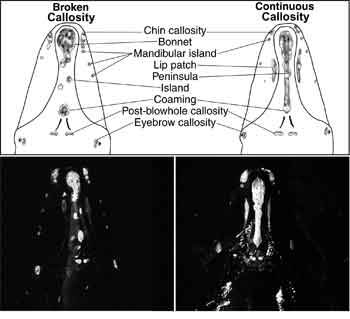
\includegraphics[width=\linewidth]{Images/callosity_comparison}
	\caption{}
	\label{fig:whale-collosity}
\end{figure}


Each whale has a set of unique
How to recognize

\subsection{Classification of images}
How to recognize objects in images, neural network, random forest

- How to recognize whales
- How to recognize objects in images
	- Neural network
	- Random Forest

\subsection{Preprocessing images}

- How to filter out background